\documentclass{article}
\usepackage{fontenc}
\usepackage{graphicx}
\usepackage{fancyhdr}
\usepackage[utf8]{inputenc}

\title{COS1004 Computer Systems Assignment 2 Part B}
\author{James Hassall, 102100517, COS10004}
\date{23 October 2019}

\pagestyle{fancy}
\lhead{James Hassall (102100517)}
\rhead{COS10004 Computer Systems Assignment 2 Part B}

\begin{document}

\maketitle

\pagebreak
\section*{Introduction}
I am trying to make the classic Rock, Paper, Scissors (RPS) game in assembly. I initially tried to make
a calculator in assembly but realise the time to implement such an application is too long. I 
decide to make RPS becasue I could make it realitively easy, where there are two inputs and 3 outputs
(including the screen). The users makes a selection either Rock, Paper or no button down for Scissors, 
then the computer will make a decision after 4 seconds and and display its answer.  An indicator LED 
will light up red or green depending if the player lost or won respectively.

\section*{Design Outline}
Physical components of the build was 2 10k ohm resistors, 2 1k Ohm resistors, 2 buttons,
2 LED's and a lot of wiring, the physical setup of the system is realitively easy due to the simplicity
of the hardware. The software components was written in FASM becasue that is what I have been taught.
The functions I have created are the 3 different actions Rock, Paper and Scissors
\begin{figure}[h]
    \centering
    \includegraphics[scale=0.7]{mainloop.png}
    \caption{The main loop}
\end{figure}
where they link up to a created function called DrawChars (located in DrawChar.asm) which will handle the drawing of the characters
on to the display.
\\
The program first waits for a user input and declares a response respectively, if the user selects scissors (e.g no input) the lights
do not turn on and declare a draw. When the user selects rock it will turn on the green LED and declare the user the winner, then if
the user selects Paper it will display a red LED indicating the user has lost.
\begin{figure}[h]
    \centering
    \includegraphics[scale=0.7]{leds.png}
    \caption{The led functions}
\end{figure}

The other functions created are just inialising the GPIO pins and defining the inplementation of the screen so the users input can view
their choice visually.


\section*{Assumptions}
I have assumed that using the GPIO reference doc that was in the earlier labs was fair to use.

\section*{Unresolved Problems}
As of current build the Ai only ever chooses Scissors and therefore the user can always win.

\pagebreak
\section*{Running Program}
\begin{figure}[h]
    \centering
    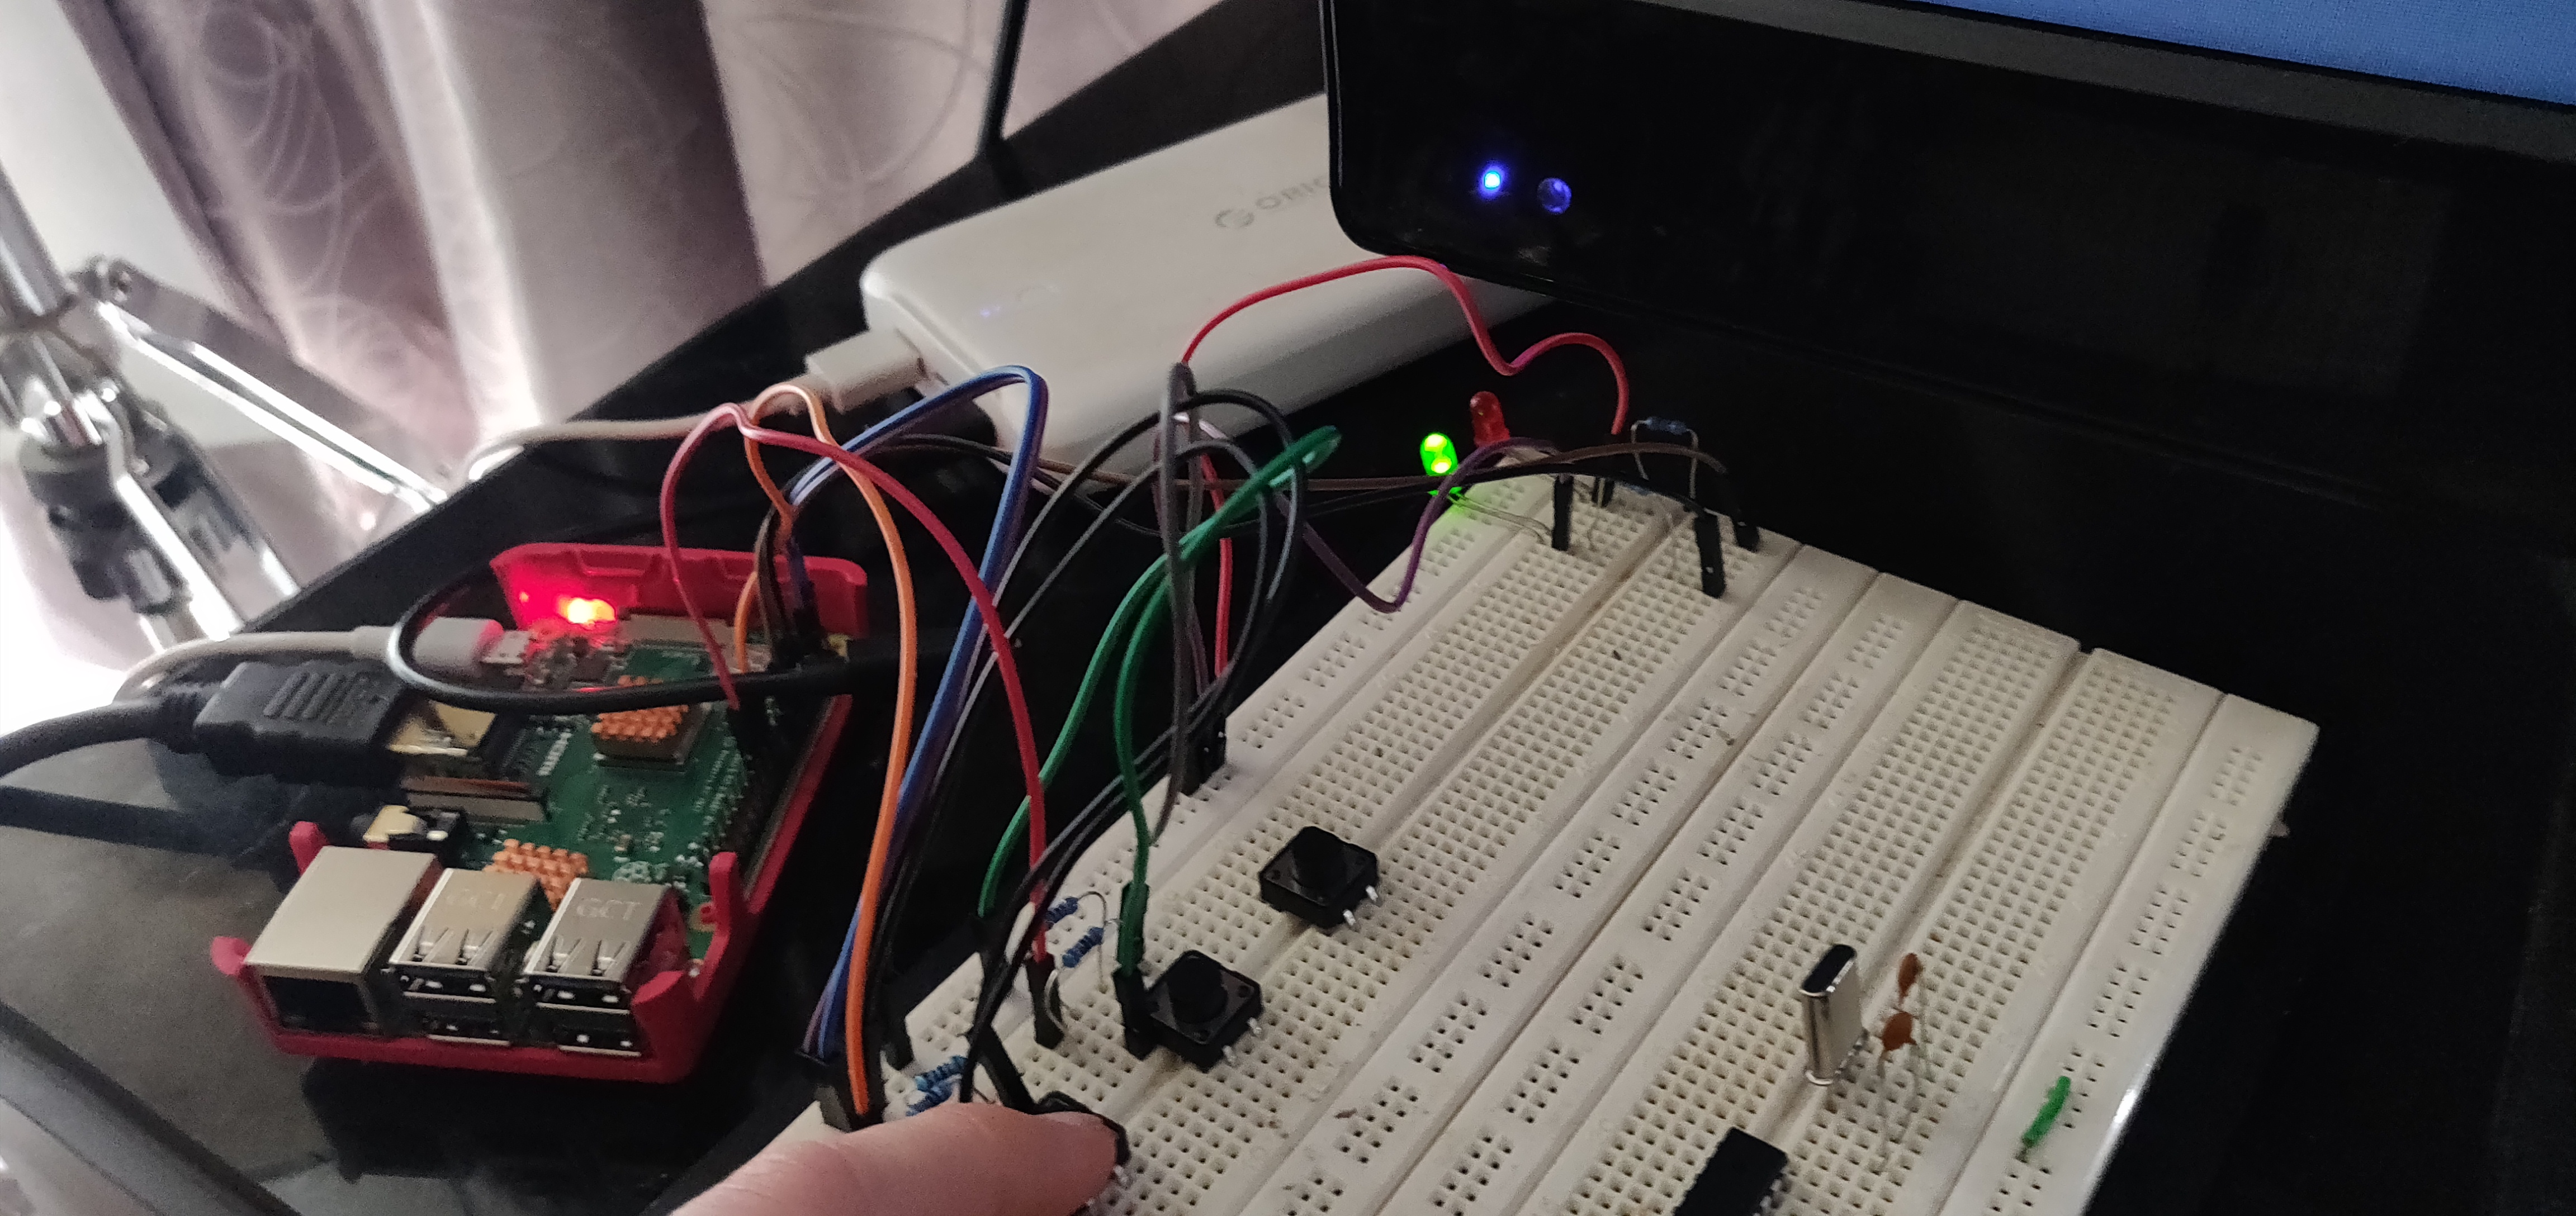
\includegraphics[scale=0.08]{ledon.jpg}
    \caption{ledon}
\end{figure}
\begin{figure}[h]
    \centering
    
\includegraphics[scale=0.08]{rock.jpg}
\end{figure}

\end{document}
